Currently, our main focus lays on the RQ1, learning, defining and differencing between software engineering practices regarding single-robot and multi-robot systems.
Our software architecture, Self-adaptive dEcentralised Robotic Architecture (SERA) is already defined.
As its name indicates, it supports a real-time decentralized robot coordination to accomplish missions with teams of robots. 
Furthermore, it is self-adaptive, responding to different changes by computing new strategies to achieve the desired goals.
SERA was already tested during an Integration Meeting of the project, where it demonstrate that can support the performance of a robot achieving different complex missions ---i.e. collaborative transportation with an human being, autonomous driving in a dynamic environment.

The aforementioned architecture is three layers architecture that is strongly influenced by the well-known work of Kramer and Magee~\cite{kramer}.
It has the same structure, but, as depicted in Figure~\ref{fig:arch}, we also added a new item that works as a central station.
It is important to remark that the aim of our project is to build a system that can be easily used by not technical users, so we had to define a way for them to command the missions to the robotic team.
The central station is just used during design-time in order to allocate a graphical interface to be used by a final user.

On the other hand, SERA follows the component-based style, so the main robotic functionalities are encapsulated in different modules or "components".
All this components are developed abstracting the communication capabilities since we rely on the interfaces defined in the architecture.
It not only significantly reduces the complexity of the code but also triggers the modularity of our system making possible exchanging the components that conform our architecture.

\begin{figure*}[!t]
\begin{center}
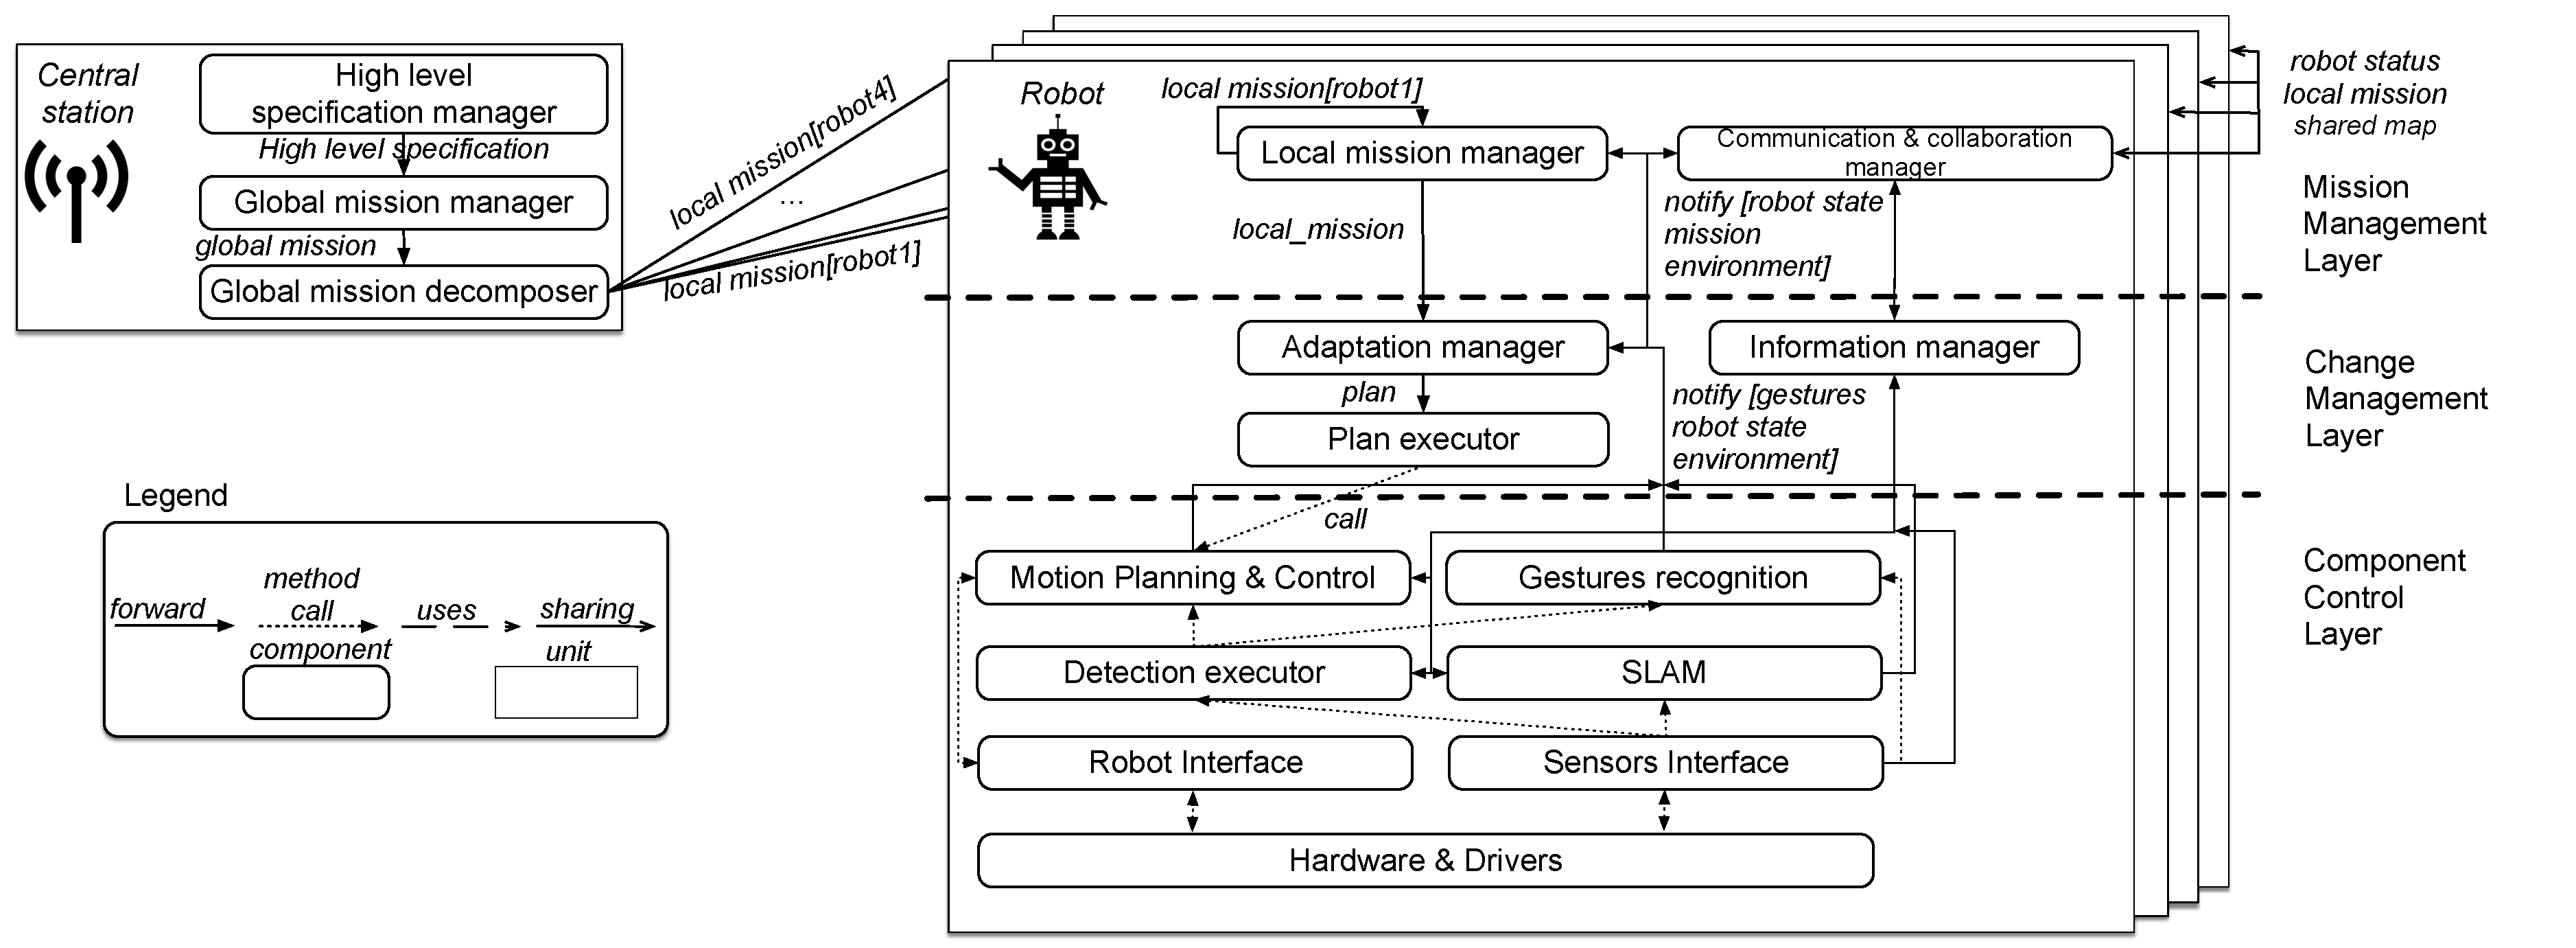
\includegraphics[width=1\linewidth]{Figures/InstanceMultiRobot_Graffle.pdf}
\caption{Software architecture.}
\label{fig:arch}
\end{center}
\end{figure*}

Since the components of our architecture are exchangeable our next short-term goal is to define configuration facilities that can be applied to our system depicted in the architecture.
It will allow to our applications to support two things:
\begin{enumerate}
\item Being customizable at design-time, so we can configure its components based on the requirements of our context (i.e. hardware installed in each robot, environment where they will be deployed, etc.)
\item To self-adapt or self-configure at run time, so each robot can apply changes in its configuration based on emergent events of the environment or failures of their system.
\end{enumerate}

In order to do so we will implement pluginlib~\footnote{http://wiki.ros.org/pluginlib}, a package that uses the ROS build infrastructure and provides tools for writing and dynamically loading plugins.

Finally, in order to communicate each robot with its teammates we implemented an approach based on ROS+REST.
So, using a suitable component that works as an interface we are able to send messages in form of services between robots.
In this way, each robot has an instance of ROS running in their own local environment so we can deploy a whole team of robots avoiding a central master node and the problems related with this approach (i.e. bottleneck issues, less robustness facing failures of a node, etc.), specially working with the ROS middleware.

